	\documentclass[12pt]{article}
\usepackage{graphicx}
\usepackage{float}
\usepackage[margin=1.0in]{geometry}
\restylefloat{figure}
	\title{IT3708 - Exercise 2}
\author{
        Eirik Hammerstad \& Nicklas Utgaard
}
				
\date{\today}
\begin{document}
\maketitle
\pagebreak
\tableofcontents
\pagebreak
\section{Description}
	\subsection{Architecture}
		\subsubsection{GA-core}
			Figure~\ref{fig:gastruct} below show the architecture of the core components for our evolutionary algorithm. The whole architecture is based around modularity and reusability, which can be seen by the classes named with italic font\footnote{SelectionMechanism, SelectionProtocol, RangeBasedSelectionMechansim, StatisticsHandler, FitnessHandler, GenoType, PhenoType, Populationgenerator, PopulationParser}. This is a plain framework for solving problems through an evolitionary process and contains just the basics implementations for each interface, e.g. the binary.
			\begin{figure}[H]
				\centerline{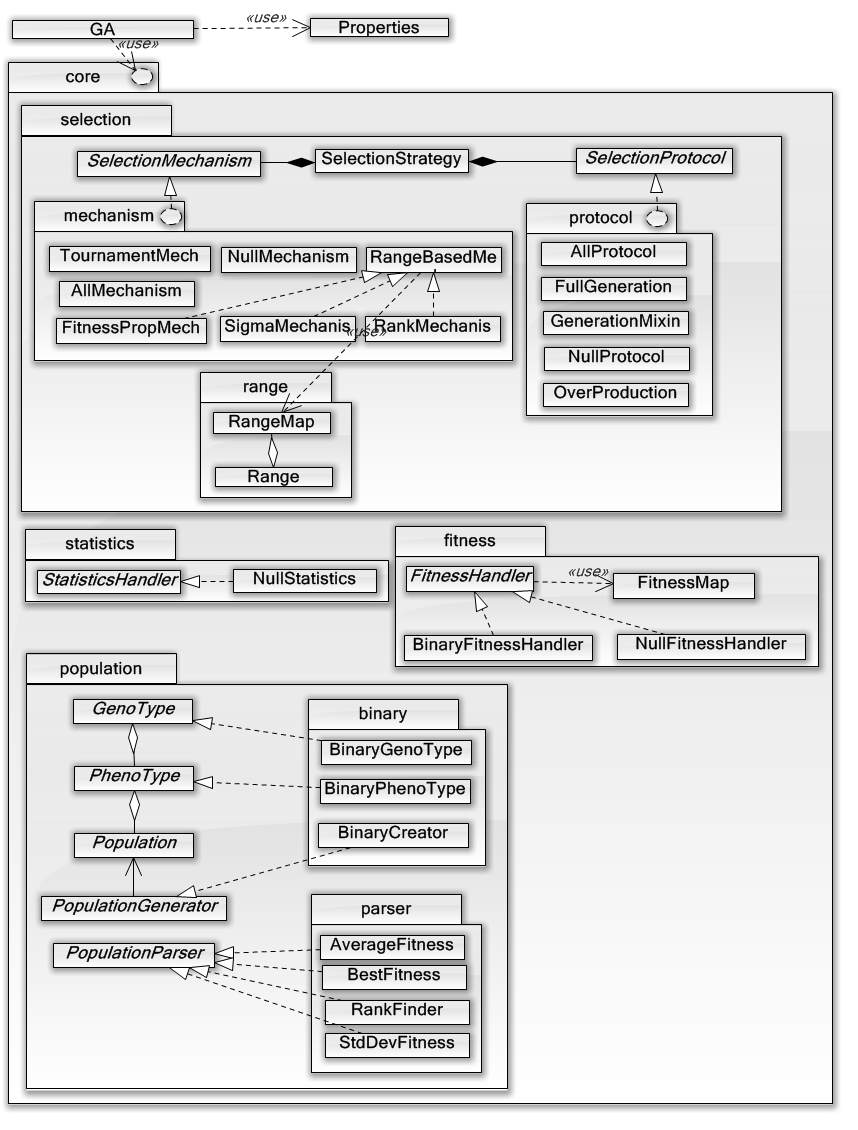
\includegraphics[width=.7\columnwidth]{./../images/GAStruct.png}}
				\caption{GA architecture}%
				\label{fig:gastruct}%
			\end{figure}
		\subsubsection{Problem specific}
		In this exercise, we implement everything problem specific in a separate project. Our SpikeGenoType, SpikePhenoType, SpikeFitnessHandler and SpikePopulationCreator extends GenoType, PhenoType, FitnessHandler and PopulationGenerator from the core project respectivly.
		Our Spike project also implements an abstraction for the SpikeTrain, including functionality for different spike train distance metrics (waveform, spike time, spike interval), reading from file, and writing to file. 
	\subsection{Genotype}
	\subsection{Fitness function}
\section{Test cases}
\section{Genotype-Phenotype mapping}
\section{Practical implications}
\section{Application in other problem domains}
\end{document}